\documentclass{beamer}
\mode<presentation>
\usepackage{amsmath,amssymb}
\usepackage{color}
\usepackage{etoolbox}
\usepackage[dutch]{babel}
\usepackage{graphicx}
\usepackage{mathtools}
\usetheme{Rochester}
\usecolortheme{beaver}
\setbeamertemplate{footline}{\insertframenumber/\inserttotalframenumber}

%\setbeamercolor{normal text}{bg=black,fg=white}
%\setbeamercolor{frametitle}{bg=black,fg=white}
%\setbeamercolor{alerted text}{bg=black,fg=white}
%\setbeamercolor{title}{bg=black,fg=white}
%\setbeamercolor{stelling}{bg=black,fg=white}

\title{Adaptieve benaderingsmethodes}
\author{Jan Westerdiep}

\newcommand{\R}{\mathbb{R}}
\newcommand{\N}{\mathbb{N}}
\newcommand{\Z}{\mathbb{Z}}
\newcommand{\C}{\mathbb{C}}
\newcommand{\A}{\mathbb{A}}
\newcommand{\Q}{\mathbb{Q}}
\newcommand{\F}{\mathbb{F}}
\newcommand{\f}{\varphi}
\newcommand{\e}{\varepsilon}
\renewcommand{\d}{\delta}

\newtheorem{bewijs}{Bewijs}
\newtheorem{voorbeeld}{Voorbeeld}
\newtheorem{stelling}{Stelling}
\newtheorem{definitie}{Definitie}
\newtheorem{gevolg}{Gevolg}
\newtheorem{opmerking}{Opmerking}

\setbeamerfont{block title}{size=\small}

\begin{document}

\begin{frame}
\titlepage
\end{frame}

\begin{frame}{Wat?}
\begin{itemize}
  \item \alert<3>{Adaptieve} \alert<2>{benaderingsmethodes} \pause
  \item Benaderen dmv.~(stuksgewijs) polynomen \pause
  \item Door in te zoomen daar waar het probleem moeilijk is \pause
  \item Dit alles adhv.~2 algoritmes van Peter Binev (2004, 2013) \pause
  \item Begeleiding door:
    \begin{enumerate}
      \item Wiskunde -- Rob Stevenson
      \item Informatica -- Dick van Albada
    \end{enumerate}
\end{itemize}
\end{frame}

\begin{frame}{$h$-verfijnend algoritme}
\begin{columns}[t]
\begin{column}[T]{\linewidth - 1.5cm}
\begin{itemize}
  \item Laat $n$ vast, $f: [a,b] \to \R$ met partitie $P = \{[a,b]\}$
  \uncover<2->{\item Partitie $P$ adaptief verfijnen, dus itereer:}
  \begin{enumerate}
    \uncover<3->{\item Voor elke $\Delta \in P$, bepaal
      \[
        e(\Delta) := \inf_{q \in \mathcal{P}^n} \| f - q\|_{L^2(\Delta)}^2 \quad \text{(Stelling: dit kan)}
      \]}
    \uncover<4->{\item \alert{Kies} $\Delta \in P$ en hak deze in twee (subdivision)}
    \uncover<5->{\item Herhaal}
  \end{enumerate}
  \uncover<6->{\item[$\Rightarrow$] Tree-Generating Algoritme}
\end{itemize}
\end{column}
\begin{column}[T]{2.5cm}
  \centering
  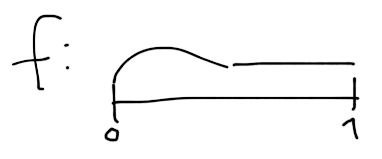
\includegraphics[width=\linewidth]{schets_0.png}\\
  \uncover<3->{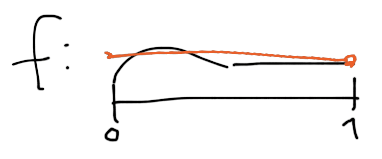
\includegraphics[width=\linewidth]{schets_1.png}\\}
  \uncover<4->{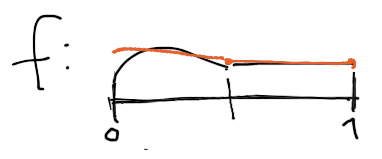
\includegraphics[width=\linewidth]{schets_2.png}\\}
  \uncover<5->{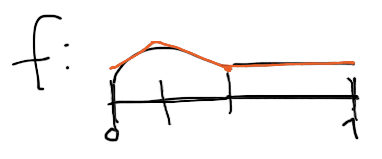
\includegraphics[width=\linewidth]{schets_3.png}\\}
\end{column}
\end{columns}
\centering
  \uncover<6->{\vspace{-1em}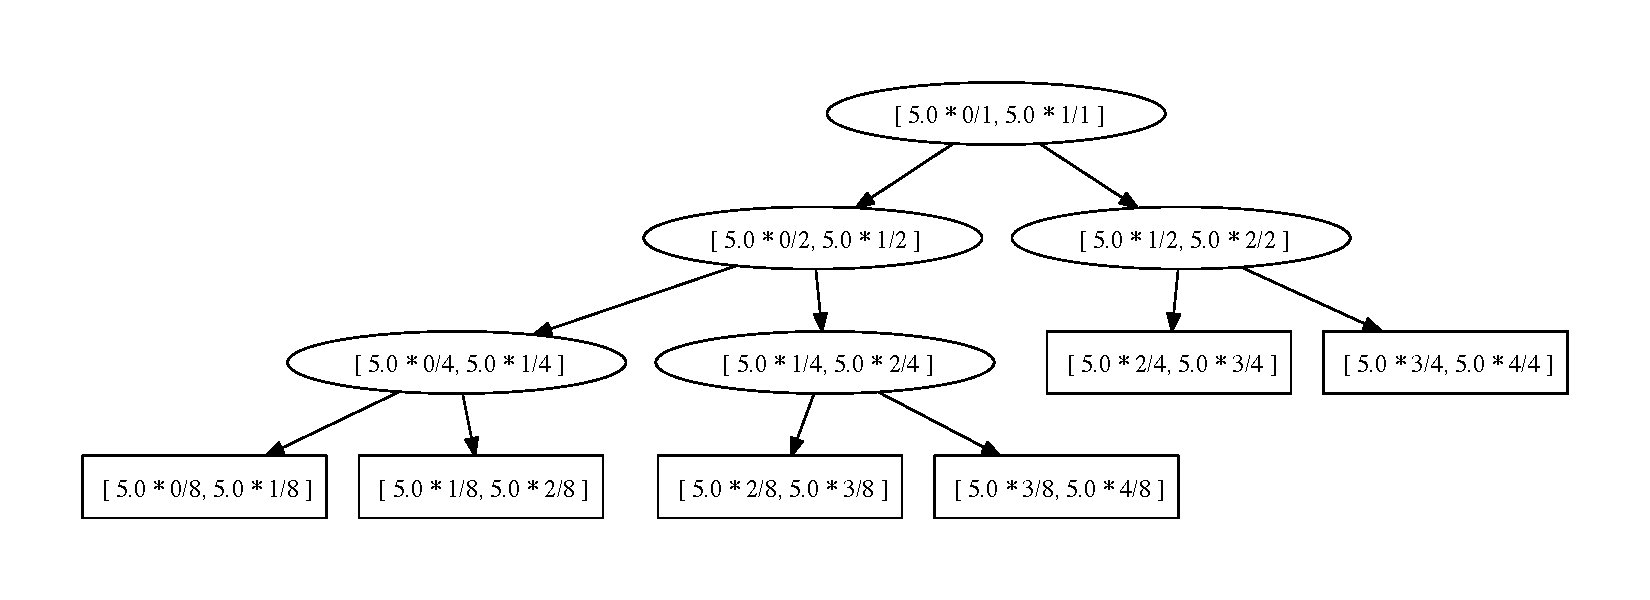
\includegraphics[width=0.8\linewidth]{lol.pdf}}
\end{frame}

\begin{frame}{$h$-verfijnende algoritmes}
\begin{enumerate}
    \item Voor elke $\Delta \in P$, bepaal
      \[
        e(\Delta) := \inf_{q \in \mathcal{P}^n} \| f - q\|_{L^2(\Delta)}^2
      \]
    \item \alert{Kies} $\Delta \in P$ en hak deze in twee (subdivision)
\end{enumerate} \pause
\begin{itemize}
  \item \emph{Greedy}: kies $\operatorname{argmax}\{ e(\Delta)\}$ \pause
  \item \emph{Binev-2004}: maak een slimmere keuze, \pause bewijsbaar:
  \item[$\Rightarrow$] Binev-2004 maakt een boom die na $n$ opdelingen \pause
  \begin{itemize}
    \item gevonden is in $\mathcal{O}(n)$ operaties, \pause en
    \item beter is dan de optimale boom in $n/2$ opdelingen
  \end{itemize}
\end{itemize}
\end{frame}

\begin{frame}{Binev-2004}
  \centering
  \only<1>{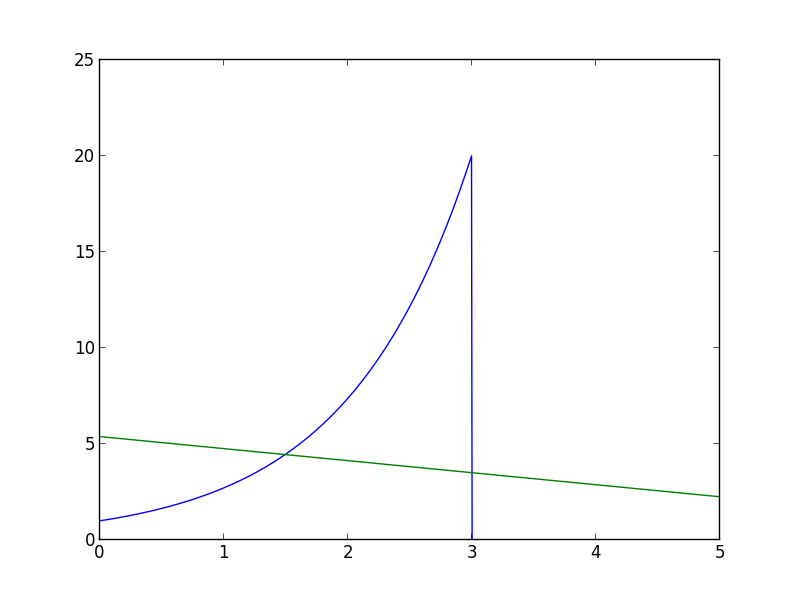
\includegraphics[height=0.5\textheight]{41.png}\\
  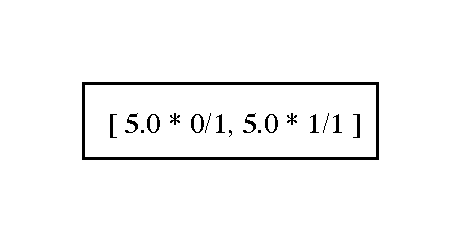
\includegraphics[height=0.5\textheight]{tree.pdf}}
  \only<2>{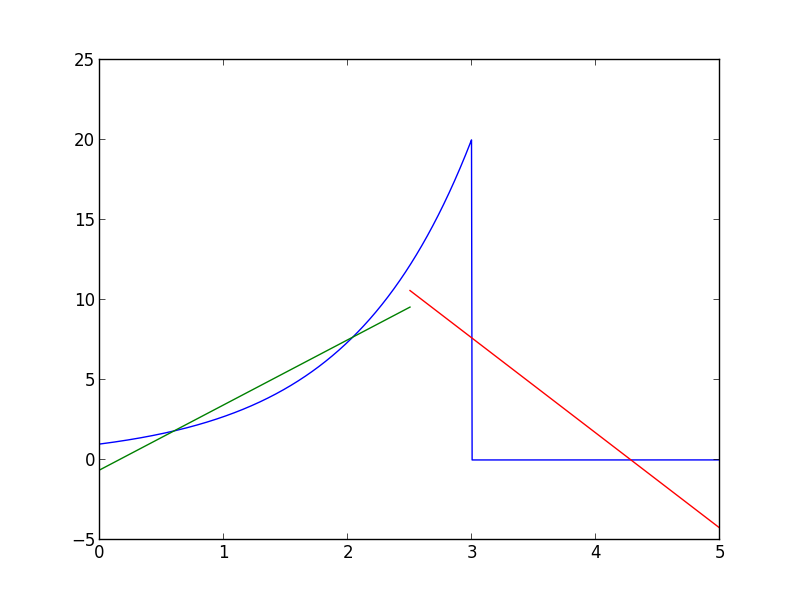
\includegraphics[height=0.5\textheight]{42.png}\\
  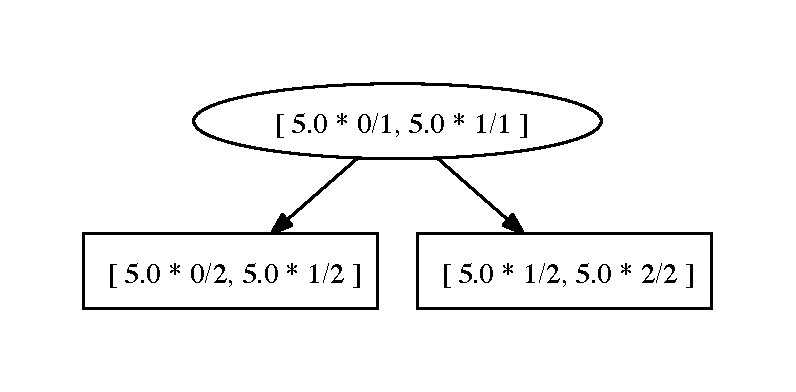
\includegraphics[height=0.5\textheight]{tree_1.pdf}}
  \only<3>{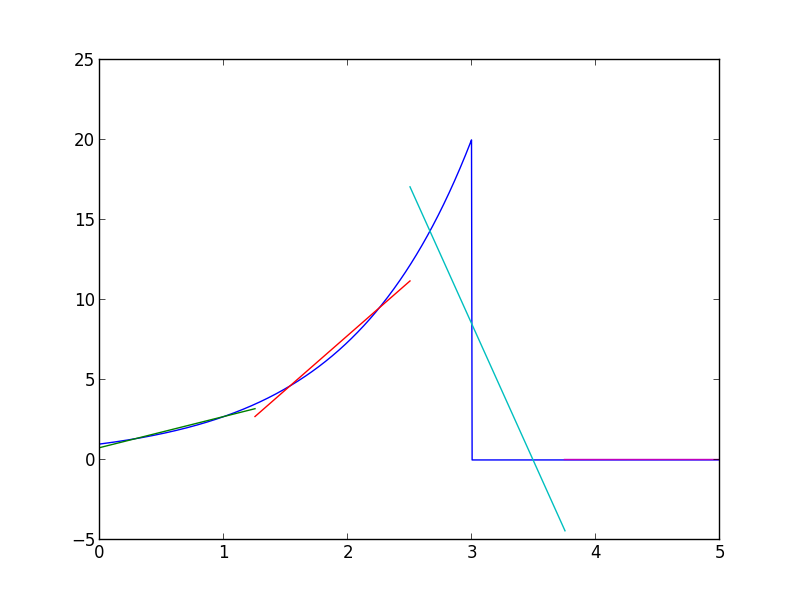
\includegraphics[height=0.5\textheight]{43.png}\\
  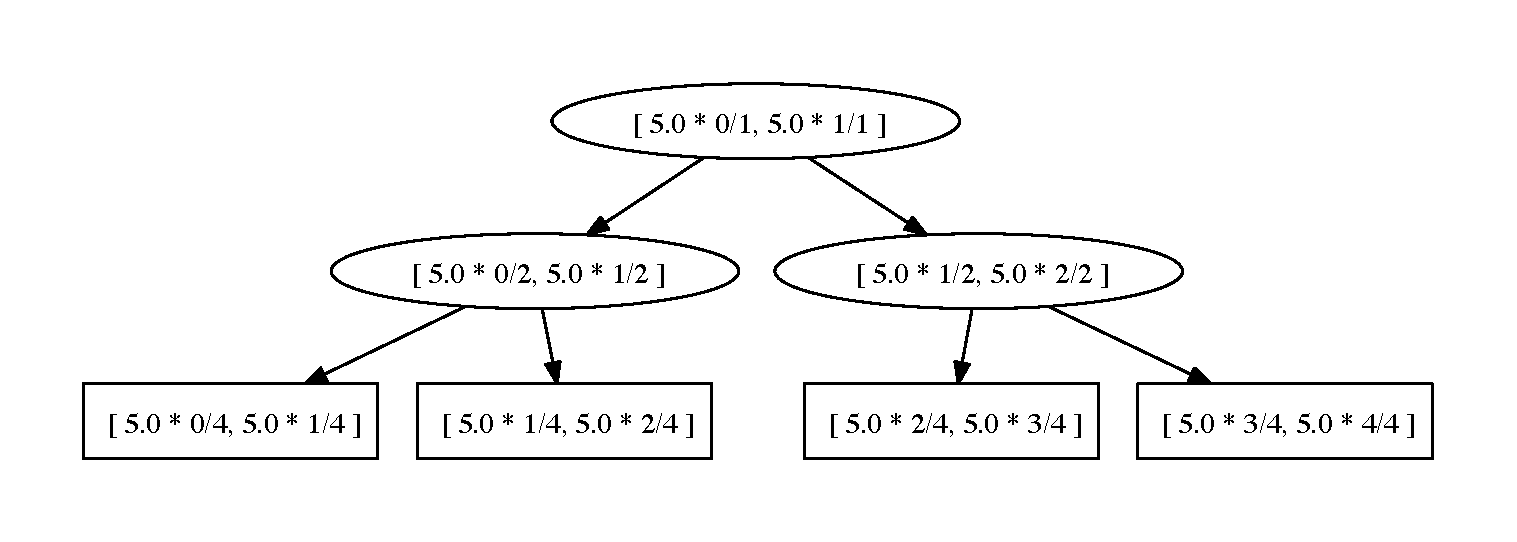
\includegraphics[height=0.5\textheight]{tree_2.pdf}}
  \only<4>{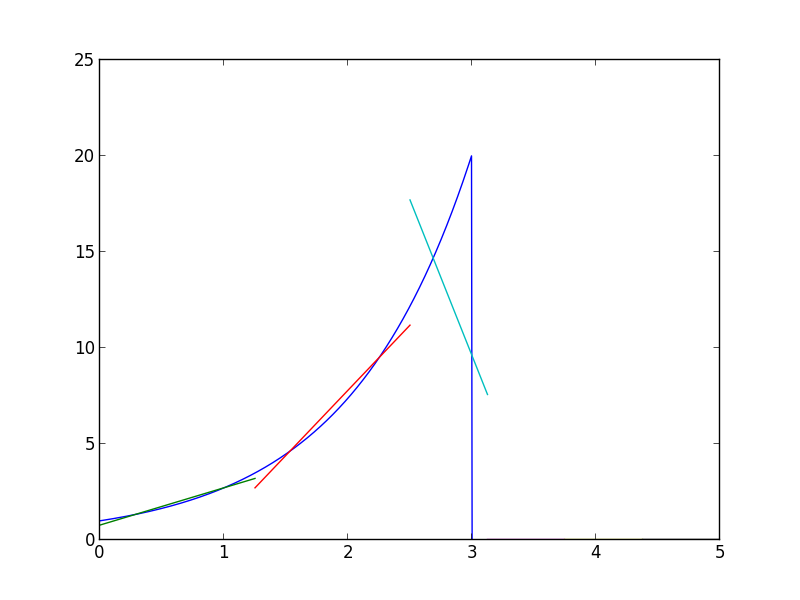
\includegraphics[height=0.5\textheight]{44.png}\\
  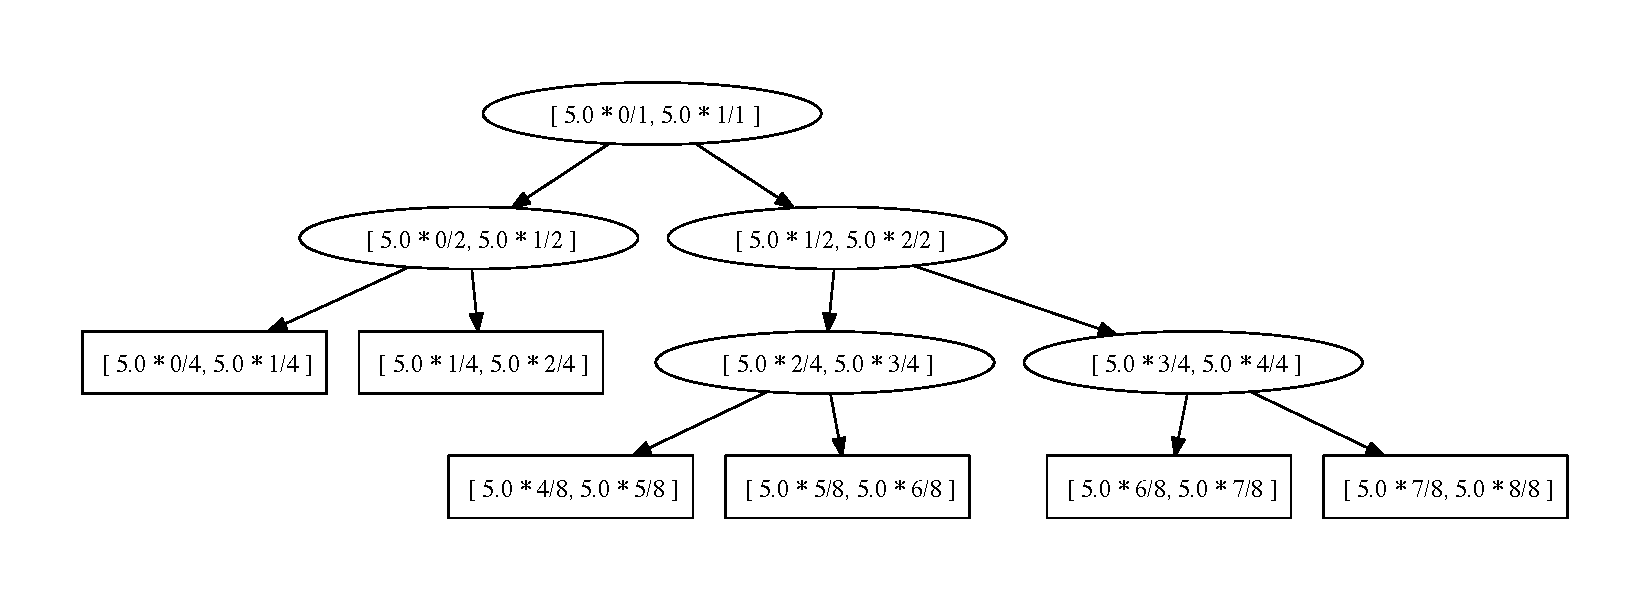
\includegraphics[height=0.5\textheight]{tree_3.pdf}}
  \only<5>{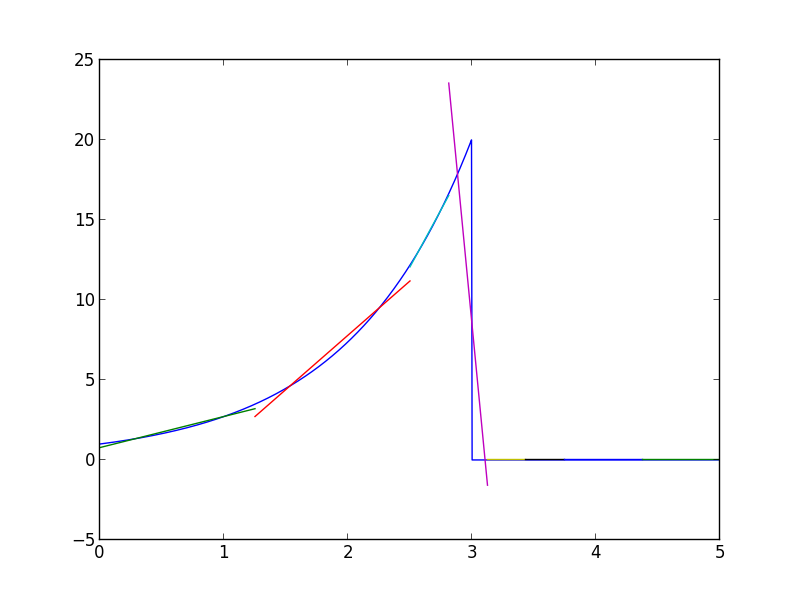
\includegraphics[height=0.5\textheight]{45.png}\\
  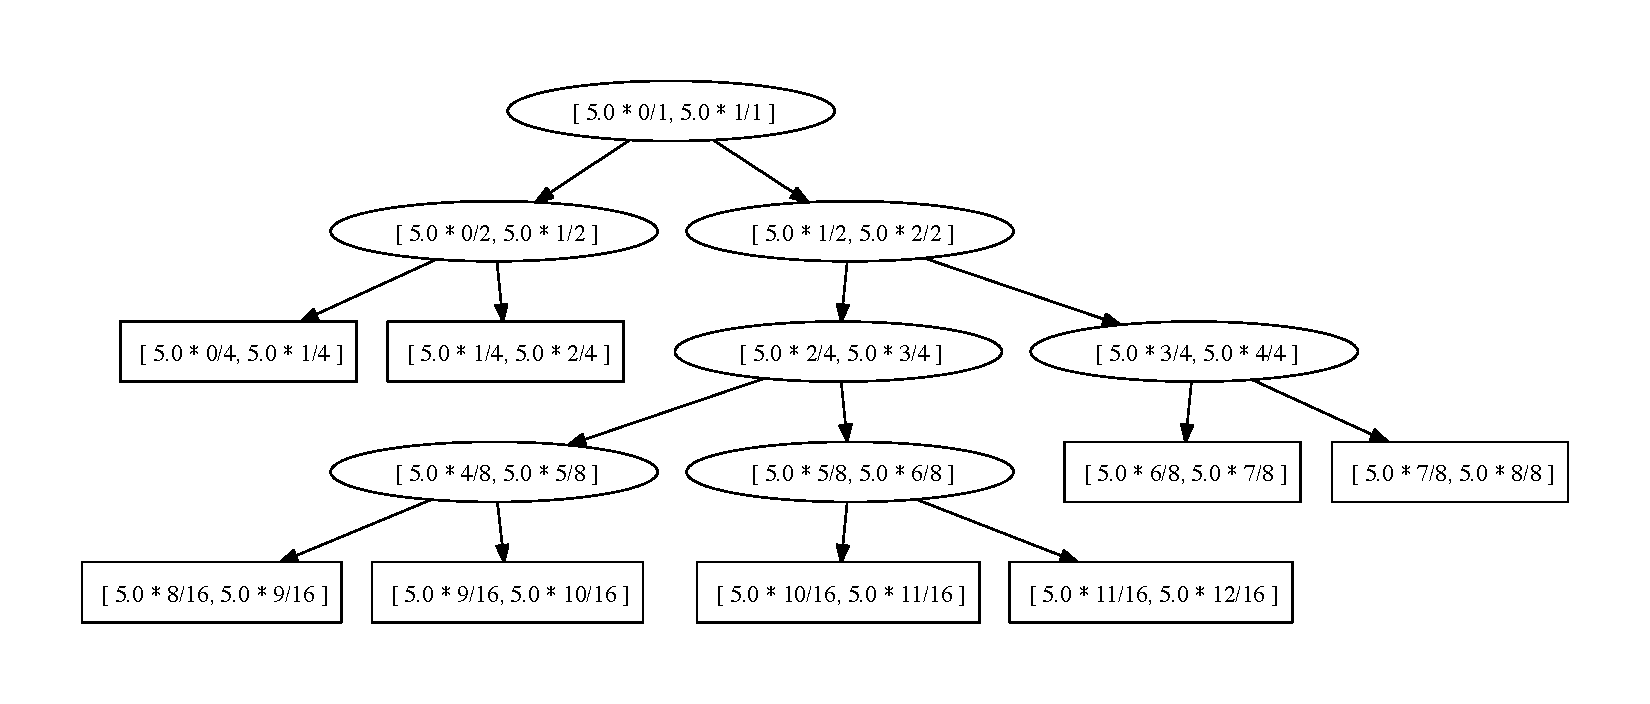
\includegraphics[height=0.5\textheight]{tree_4.pdf}}
  \only<6>{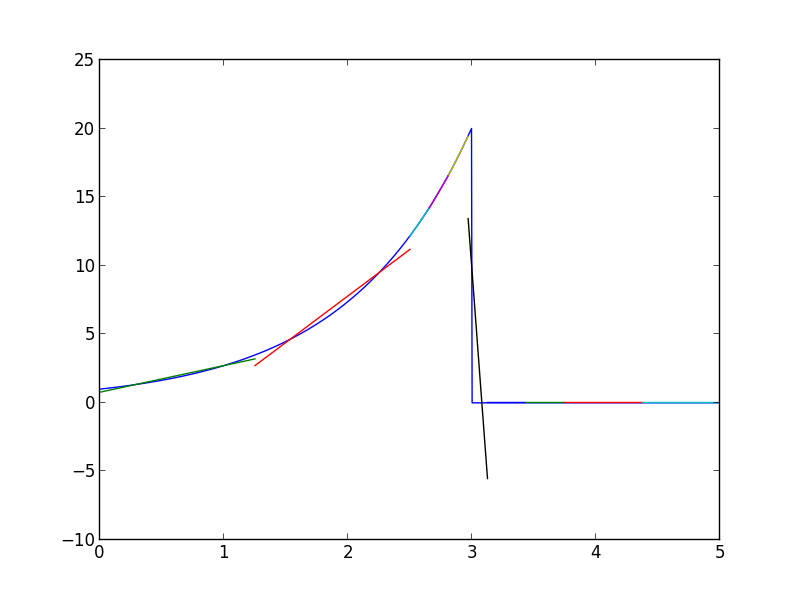
\includegraphics[height=0.5\textheight]{46.png}\\
  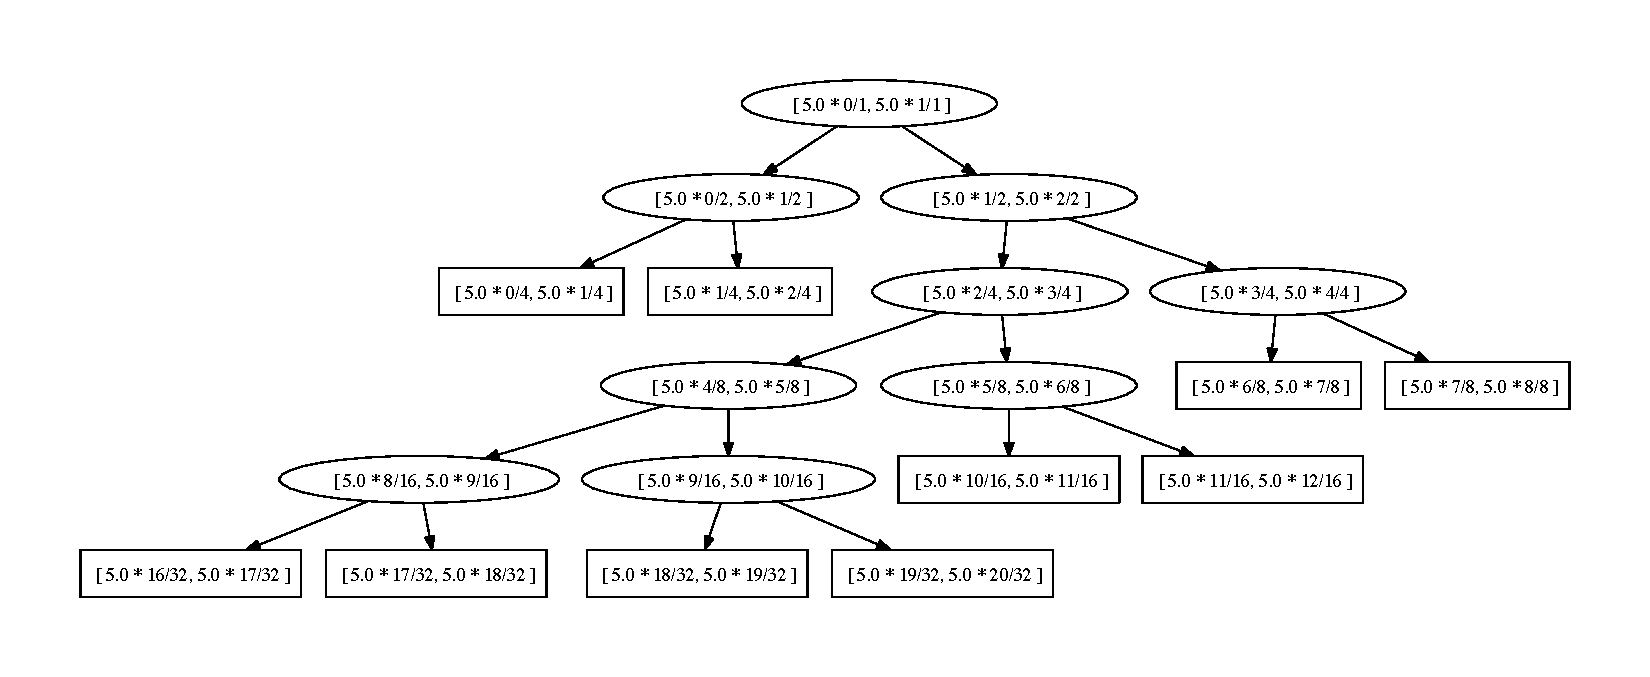
\includegraphics[height=0.5\textheight]{tree_5.pdf}}
  \only<7>{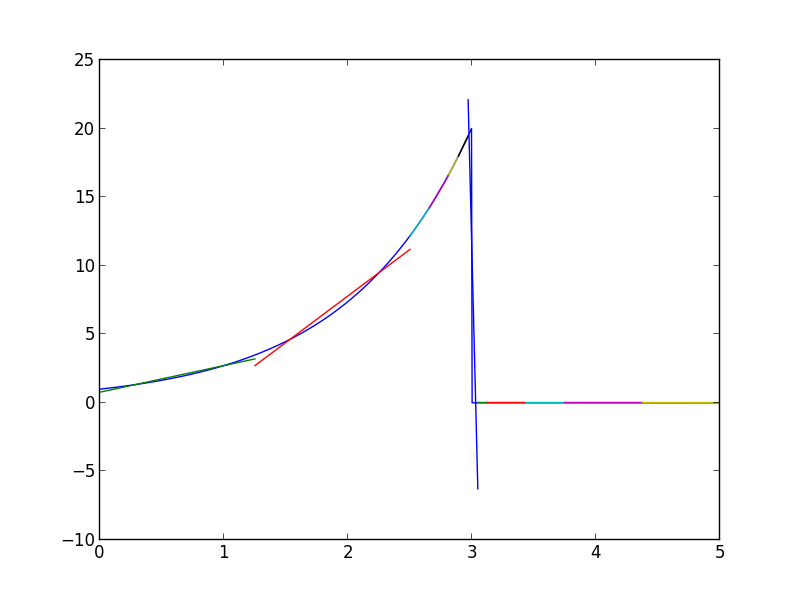
\includegraphics[height=0.5\textheight]{47.png}\\
  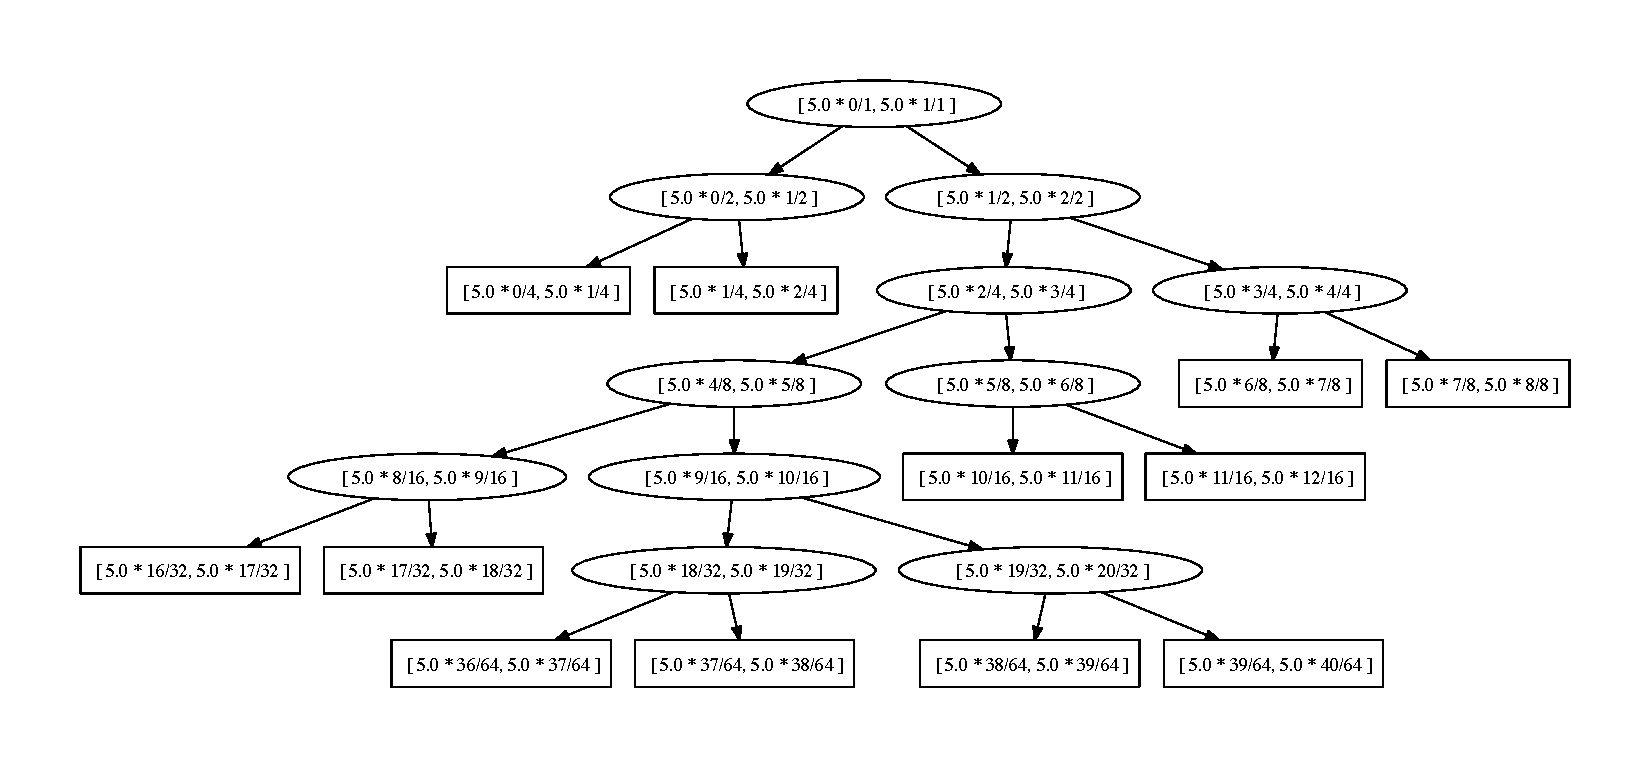
\includegraphics[height=0.5\textheight]{tree_6.pdf}}
  \only<8>{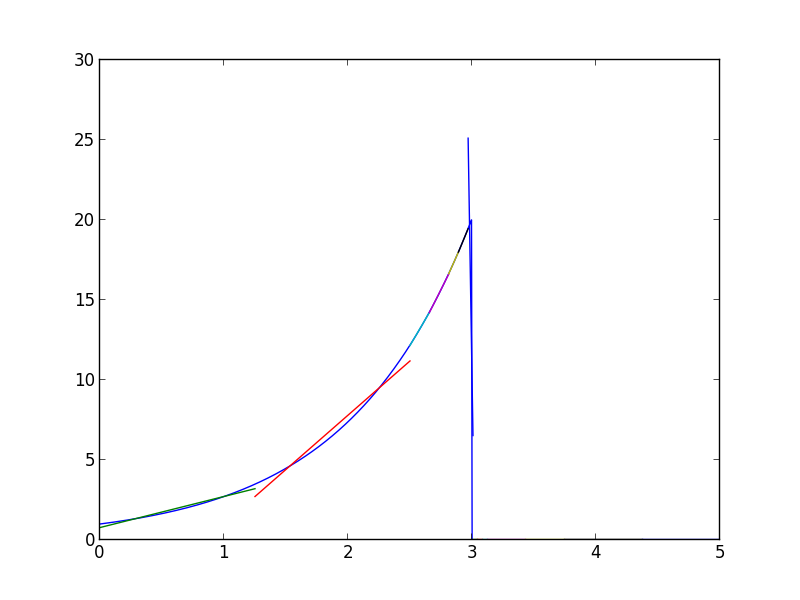
\includegraphics[height=0.5\textheight]{48.png}\\
  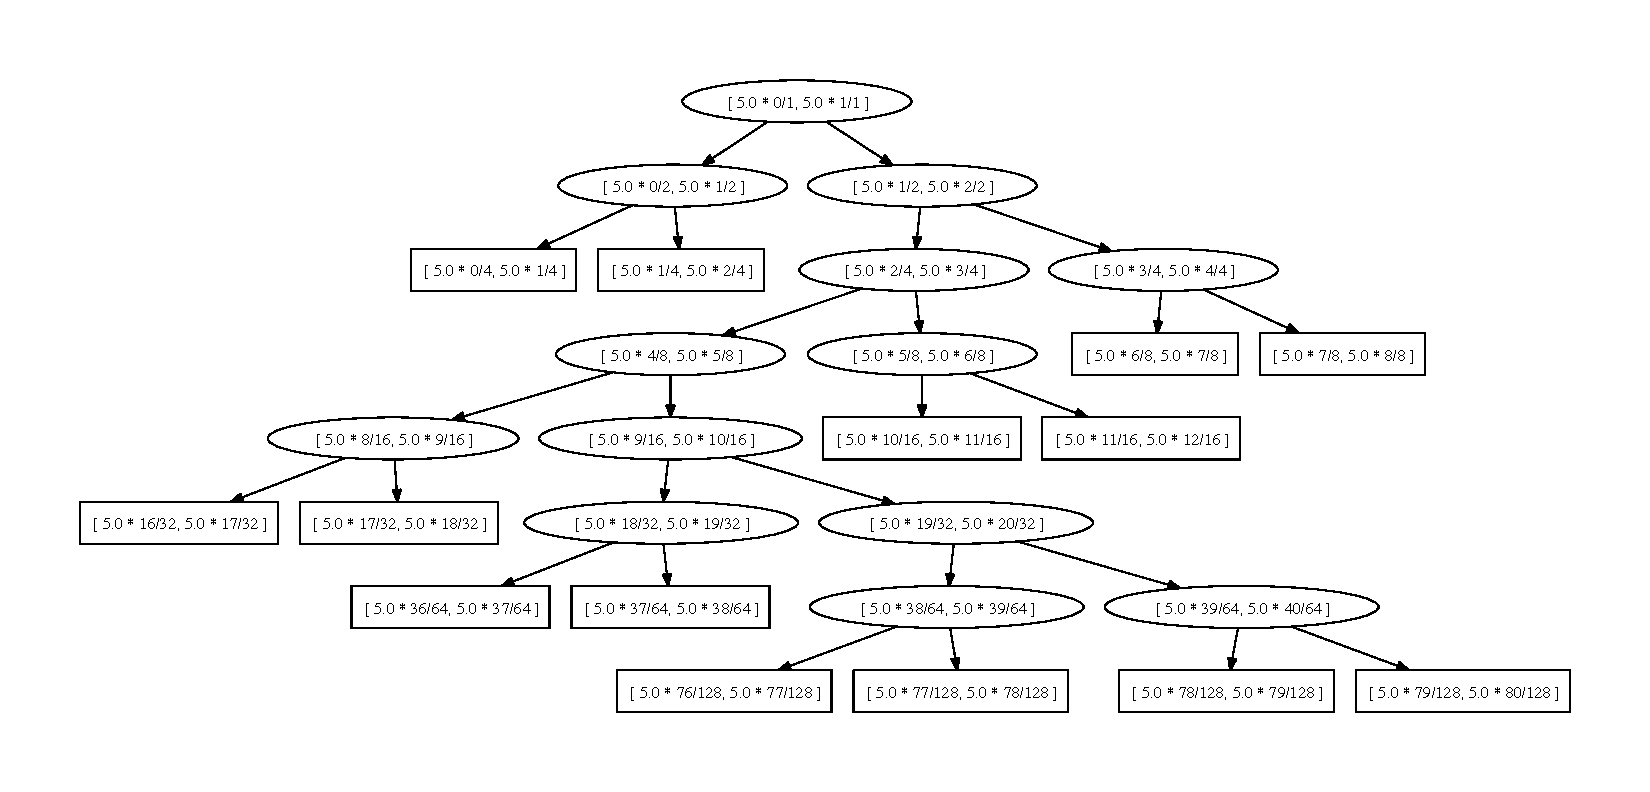
\includegraphics[height=0.5\textheight]{tree_7.pdf}}
\end{frame}

\begin{frame}{$hp$-verfijnend algoritme}
\begin{columns}[t]
\begin{column}[T]{\linewidth - 1.5cm}
\begin{itemize}
  \item Naast partitie verfijnen nu ook polynomiale graad verhogen
  \uncover<2->{\item $f: [a,b] \to \R$ met partitie $P = \{[a,b]\}$}
  \uncover<3->{\item Partitie $P$ adaptief verfijnen, dus itereer:}
  \begin{enumerate}
    \uncover<4->{\item Voor elke $\Delta \in P$, bepaal
      \[
        e_{n(\Delta)}(\Delta) := \inf_{q \in \mathcal{P}^{n(\Delta)}} \| f - q\|_{L^2(\Delta)}^2
      \]}
    \uncover<5->{\item \alert{Kies} $\Delta \in P$ en hak deze in twee (subdivision)}
    \uncover<7->{\item[$\Rightarrow$] \alert{Of} verhoog $n(\Delta)$}
    \uncover<6->{\item Herhaal}
  \end{enumerate}
\end{itemize}
\end{column}
\begin{column}[T]{2.5cm}
  \centering
  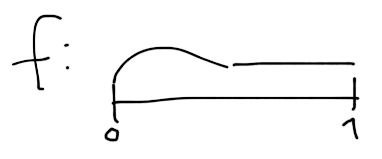
\includegraphics[width=\linewidth]{schets_0.png}\\
  \uncover<4->{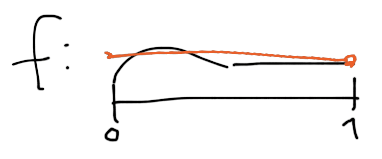
\includegraphics[width=\linewidth]{schets_1.png}\\}
  \uncover<5->{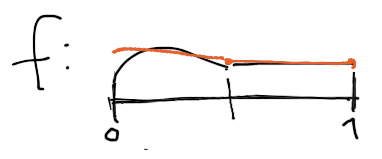
\includegraphics[width=\linewidth]{schets_2.png}\\}
  \only<6>{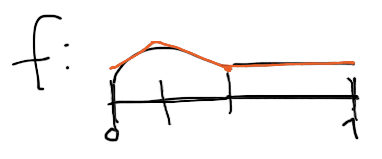
\includegraphics[width=\linewidth]{schets_3.png}\\}
  \uncover<7->{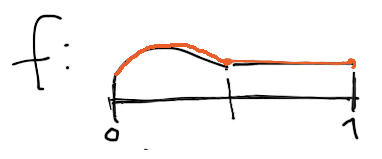
\includegraphics[width=\linewidth]{schets_4.png}\\}
\end{column}
\end{columns}
\end{frame}

\begin{frame}{Binev-2013}
  \centering
  \only<1>{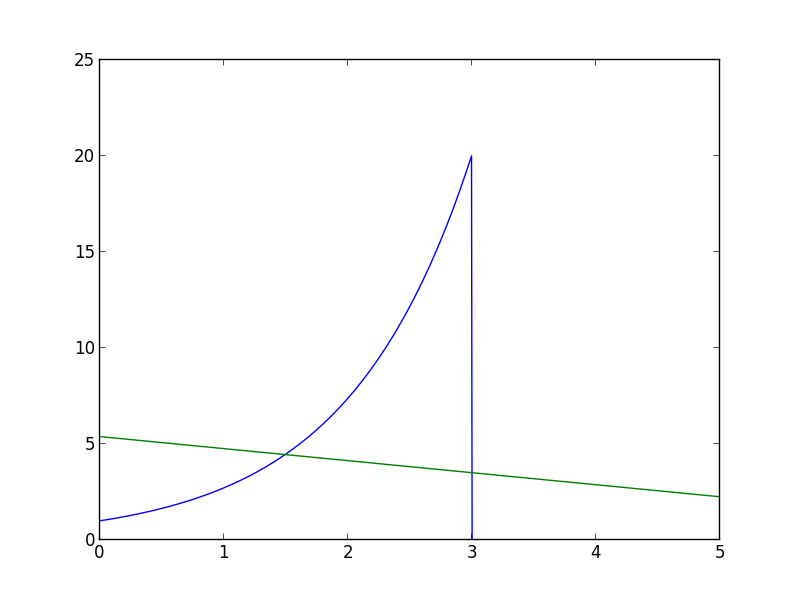
\includegraphics[height=0.5\textheight]{31.png}\\
  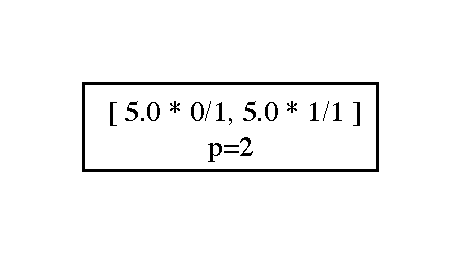
\includegraphics[height=0.5\textheight]{tree_hp_1.pdf}}
  \only<2>{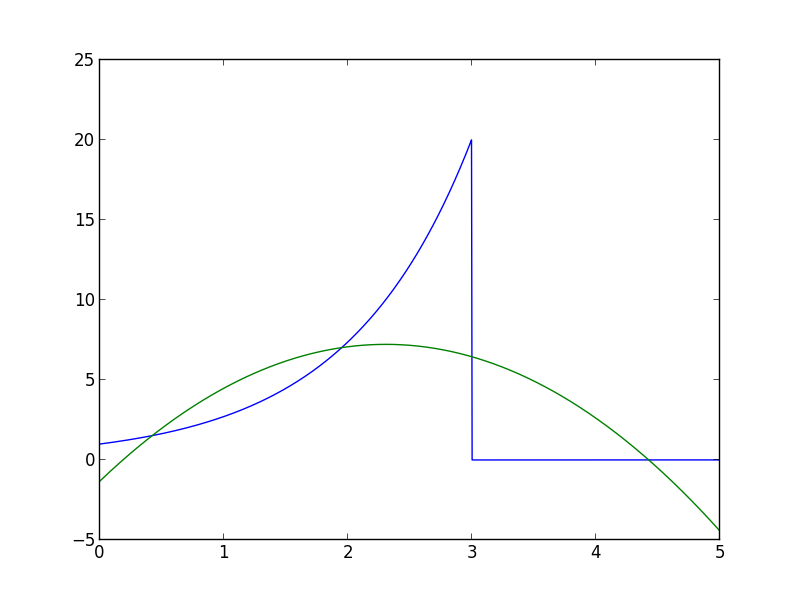
\includegraphics[height=0.5\textheight]{32.png}\\
  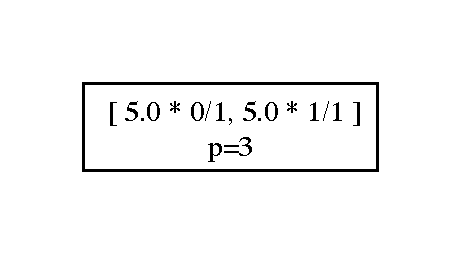
\includegraphics[height=0.5\textheight]{tree_hp_2.pdf}}
  \only<3>{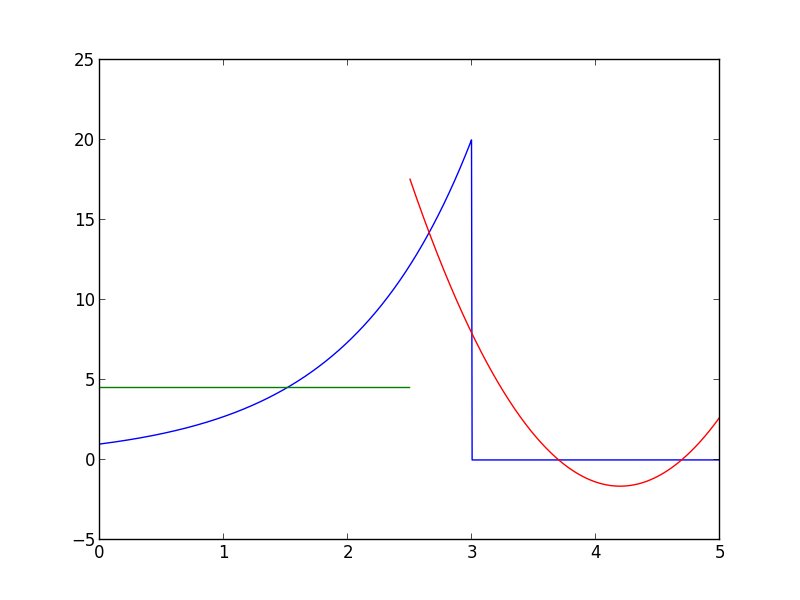
\includegraphics[height=0.5\textheight]{33.png}\\
  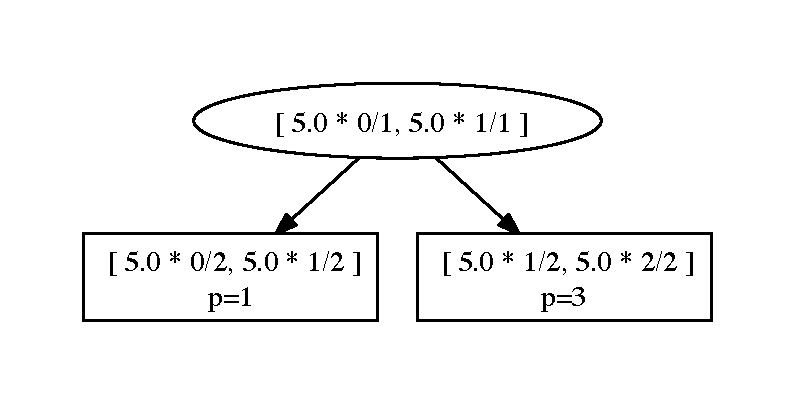
\includegraphics[height=0.5\textheight]{tree_hp_3.pdf}}
  \only<4>{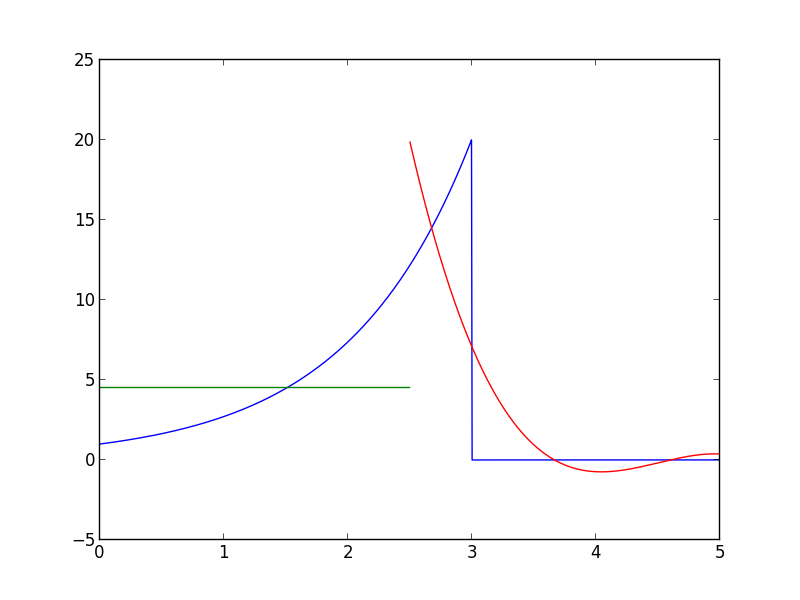
\includegraphics[height=0.5\textheight]{34.png}\\
  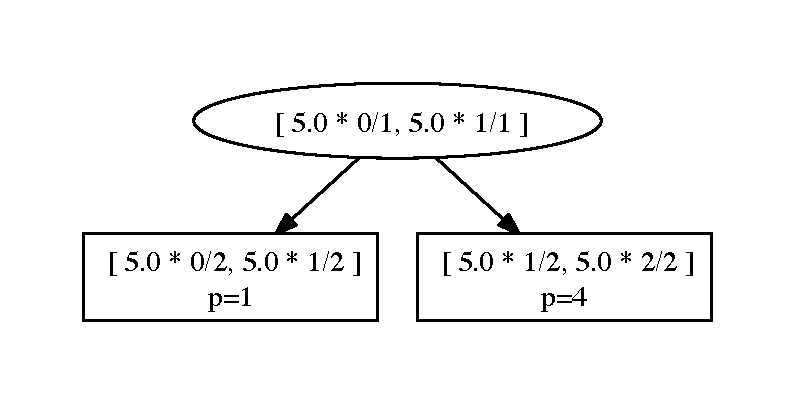
\includegraphics[height=0.5\textheight]{tree_hp_4.pdf}}
  \only<5>{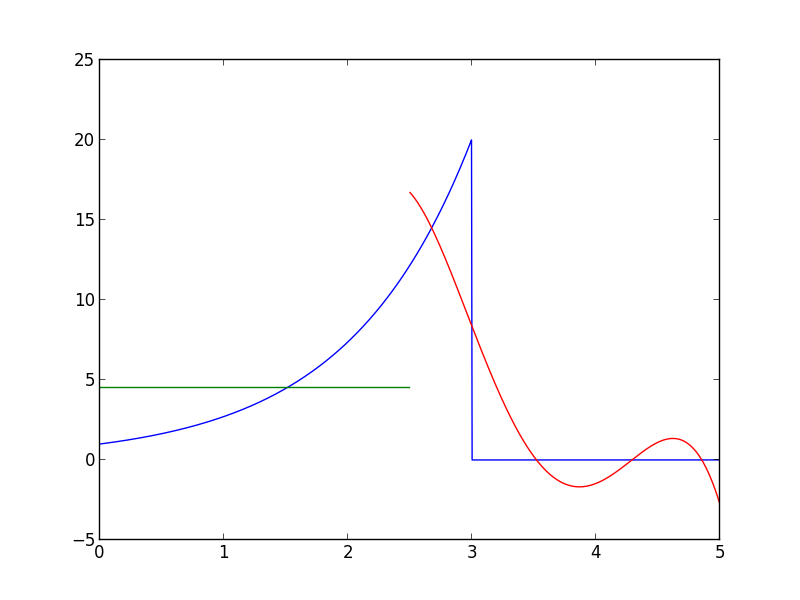
\includegraphics[height=0.5\textheight]{35.png}\\
  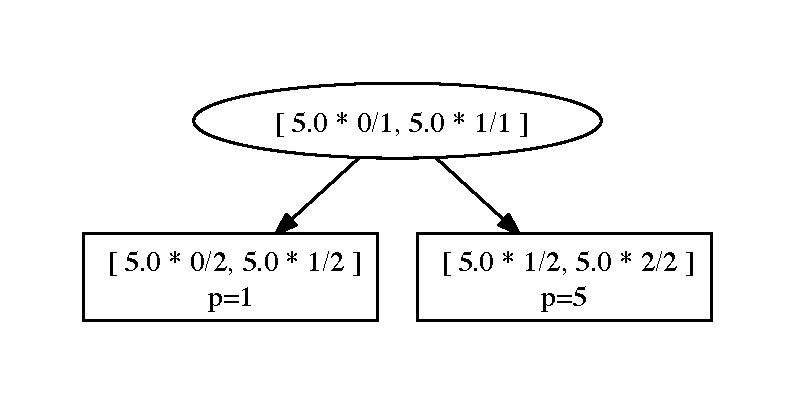
\includegraphics[height=0.5\textheight]{tree_hp_5.pdf}}
  \only<6>{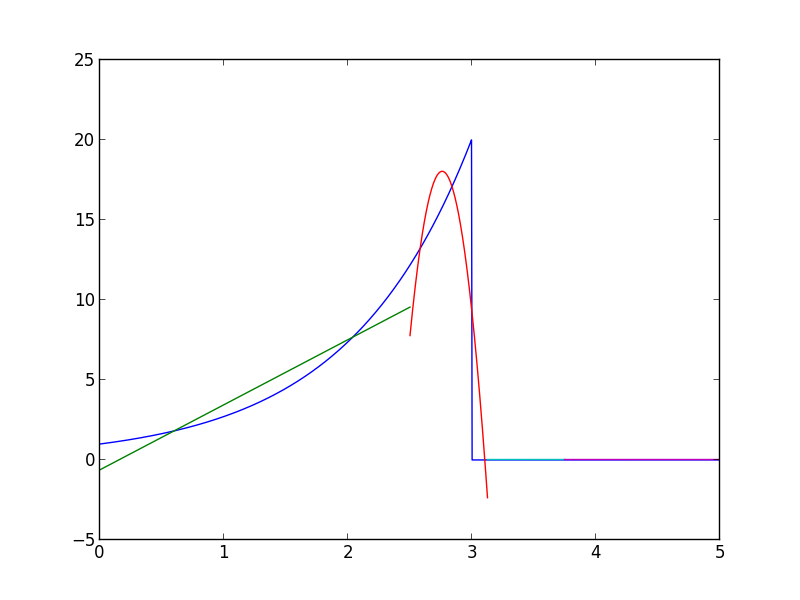
\includegraphics[height=0.5\textheight]{36.png}\\
  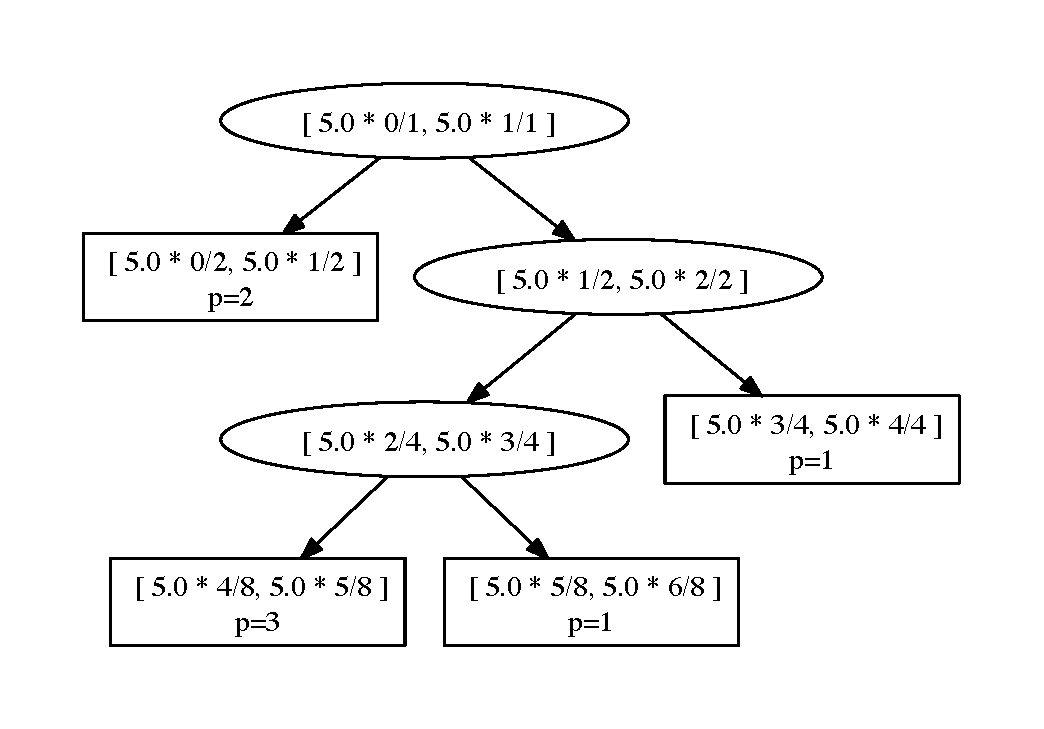
\includegraphics[height=0.5\textheight]{tree_hp_6.pdf}}
  \only<7>{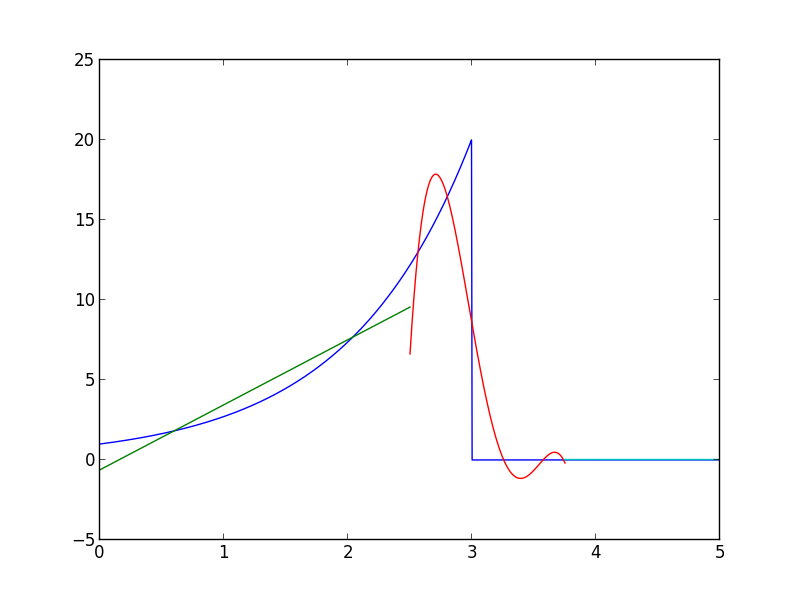
\includegraphics[height=0.5\textheight]{37.png}\\
  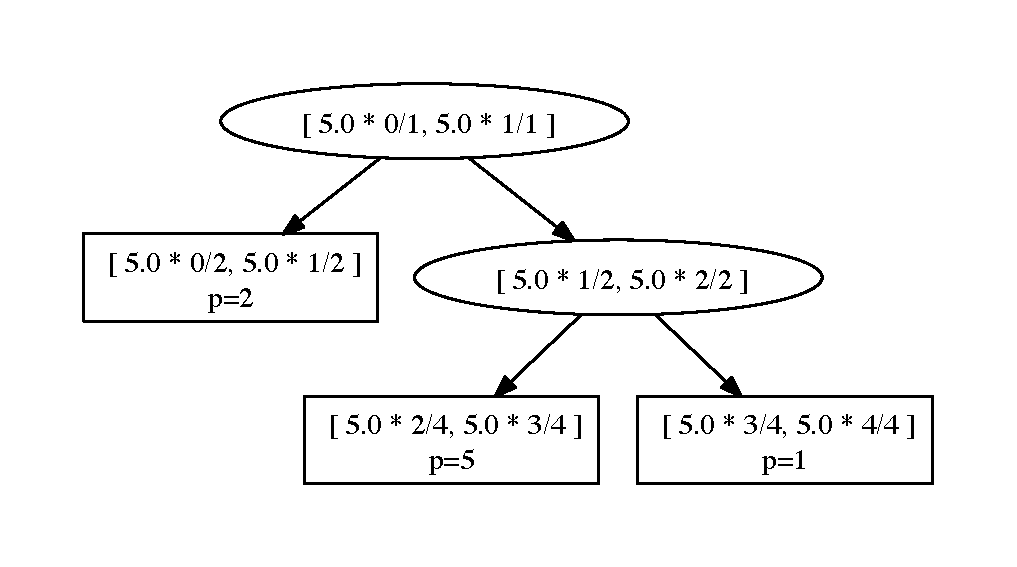
\includegraphics[height=0.5\textheight]{tree_hp_7.pdf}}
  \only<8>{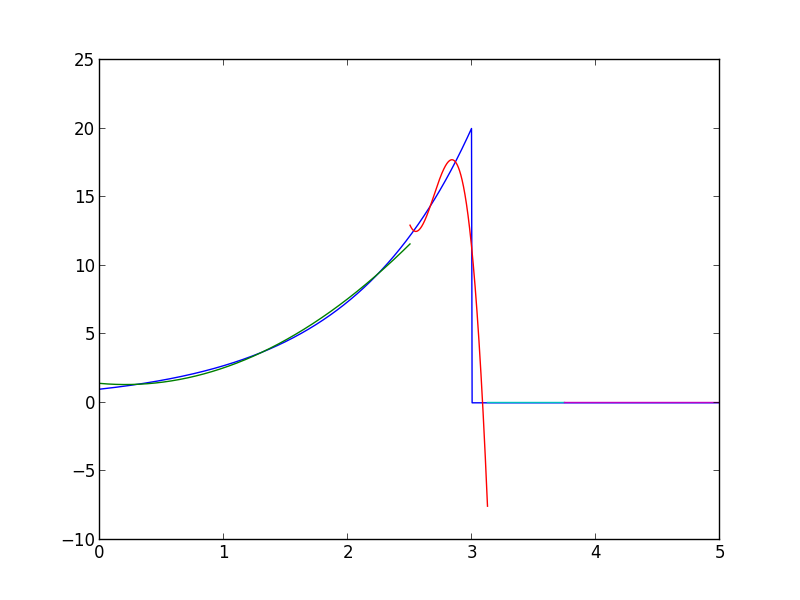
\includegraphics[height=0.5\textheight]{38.png}\\
  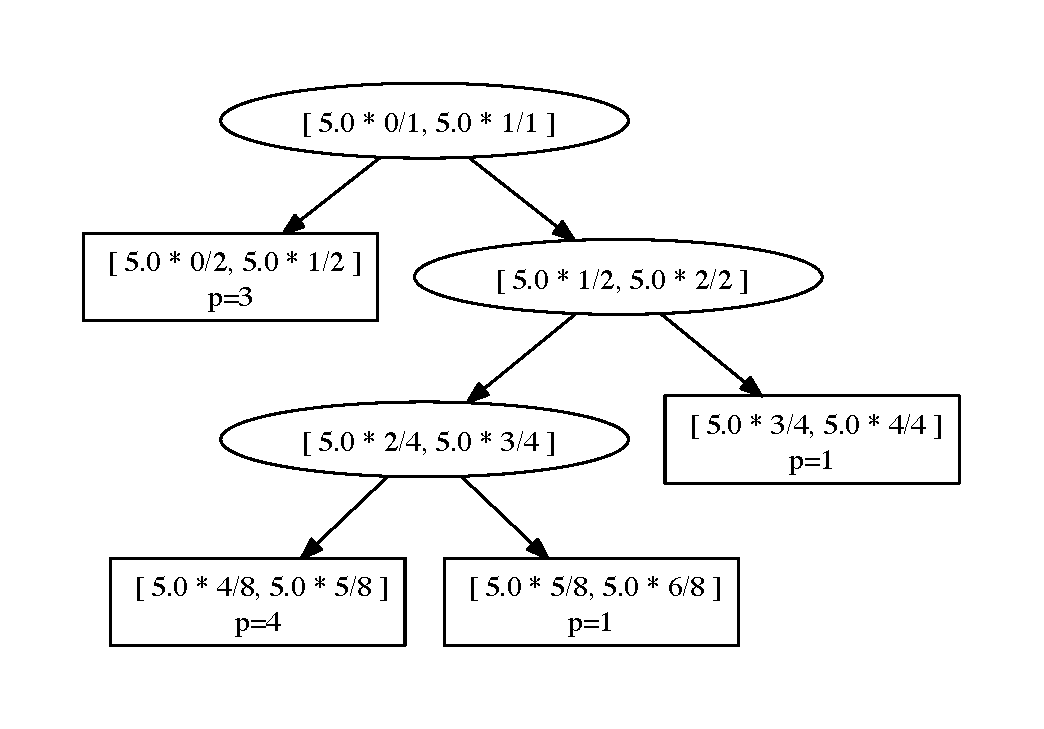
\includegraphics[height=0.5\textheight]{tree_hp_8.pdf}}
\end{frame}

\begin{frame}{Ander voorbeeld}
  \centering
  \only<1>{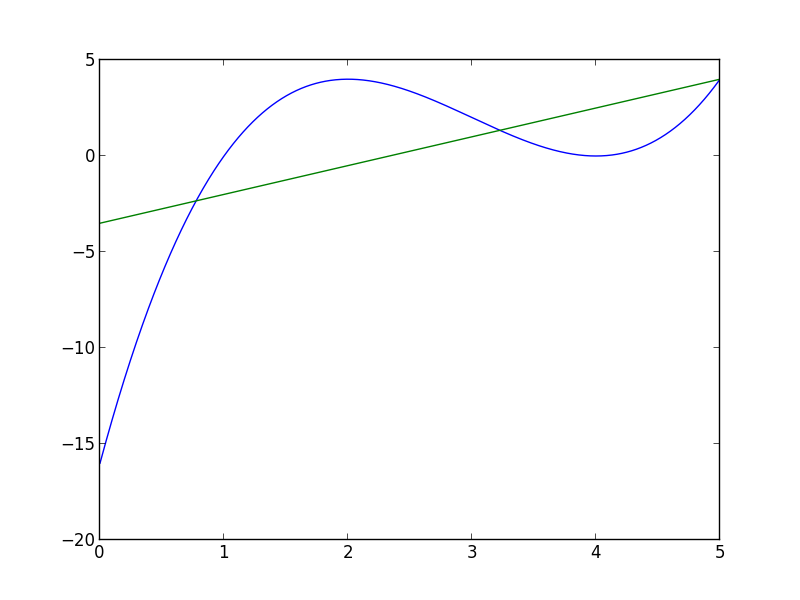
\includegraphics[width=0.5\linewidth]{11.png}
  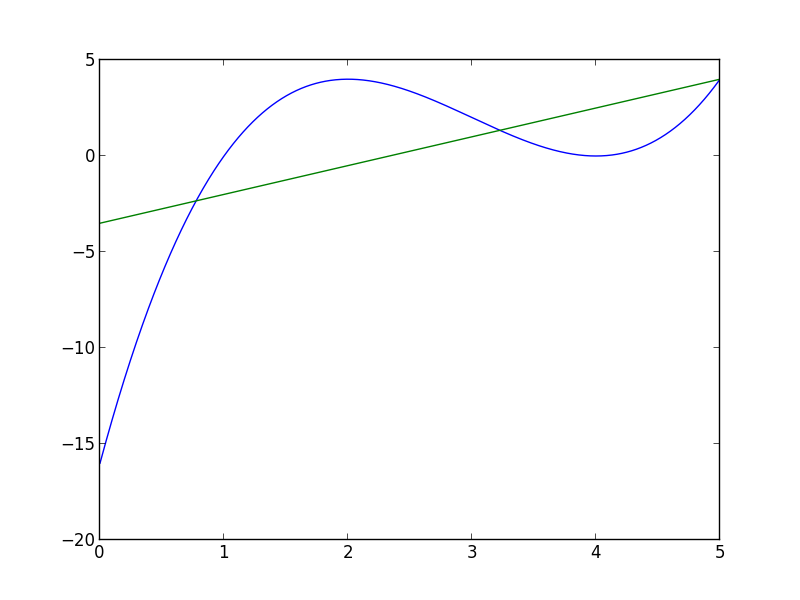
\includegraphics[width=0.5\linewidth]{21.png}}
  \only<2>{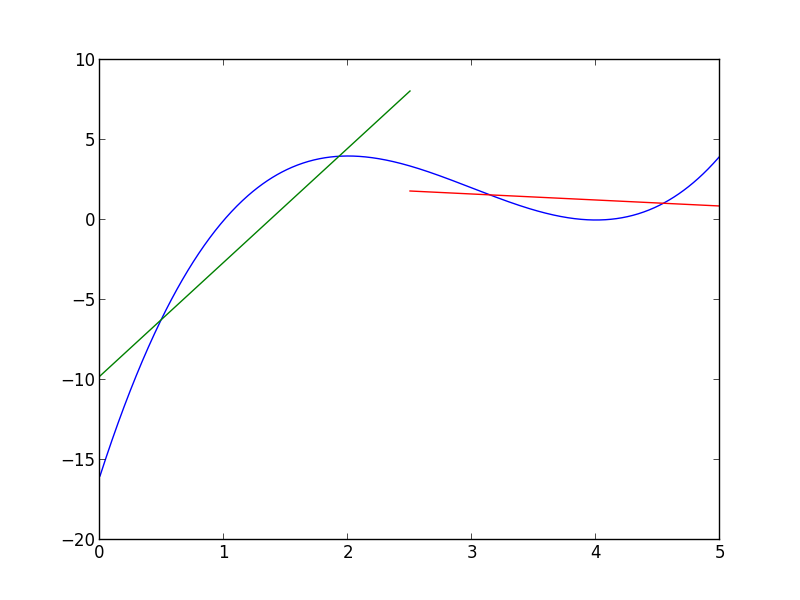
\includegraphics[width=0.5\linewidth]{12.png}
  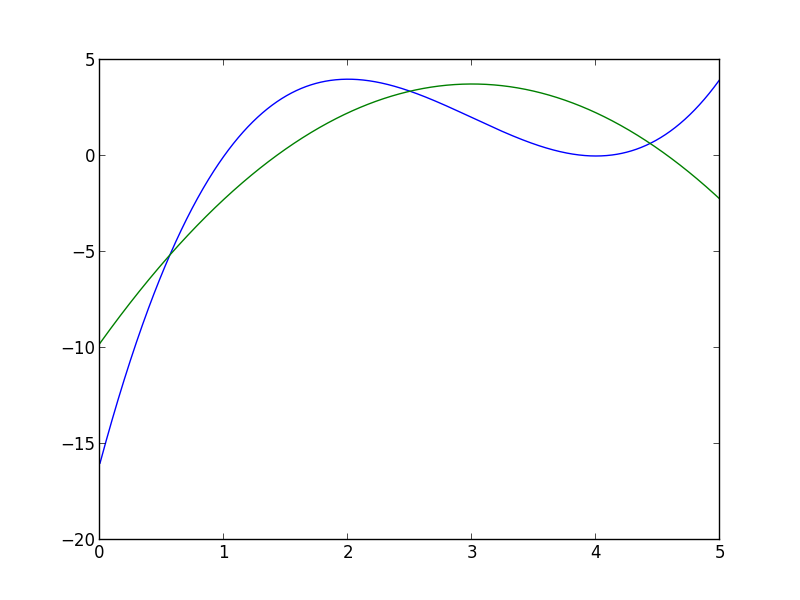
\includegraphics[width=0.5\linewidth]{22.png}}
  \only<3>{\vspace{-1em}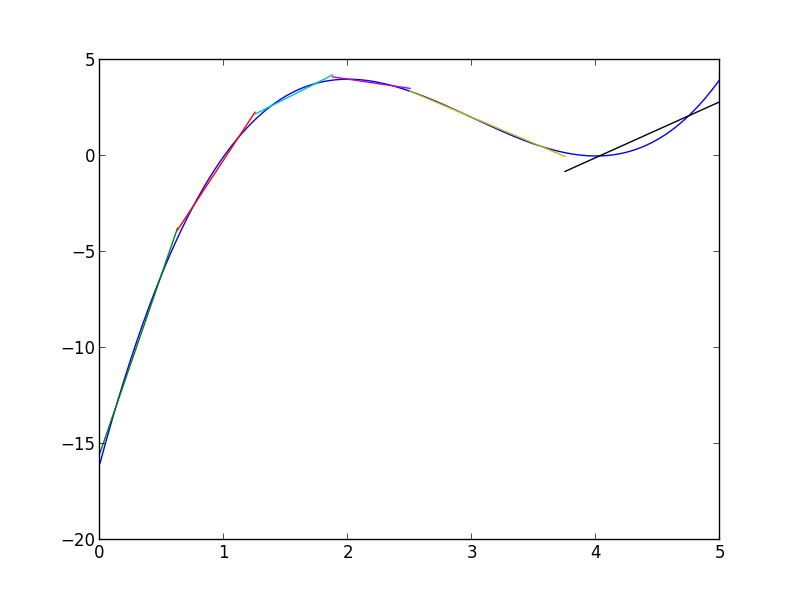
\includegraphics[width=0.5\linewidth]{14.png}
  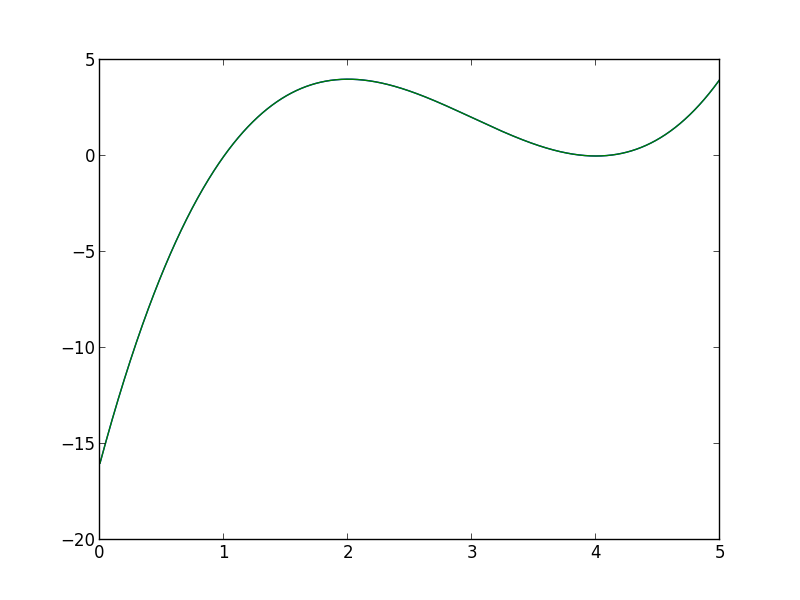
\includegraphics[width=0.5\linewidth]{24.png}}
  \only<4>{\vspace{-1em}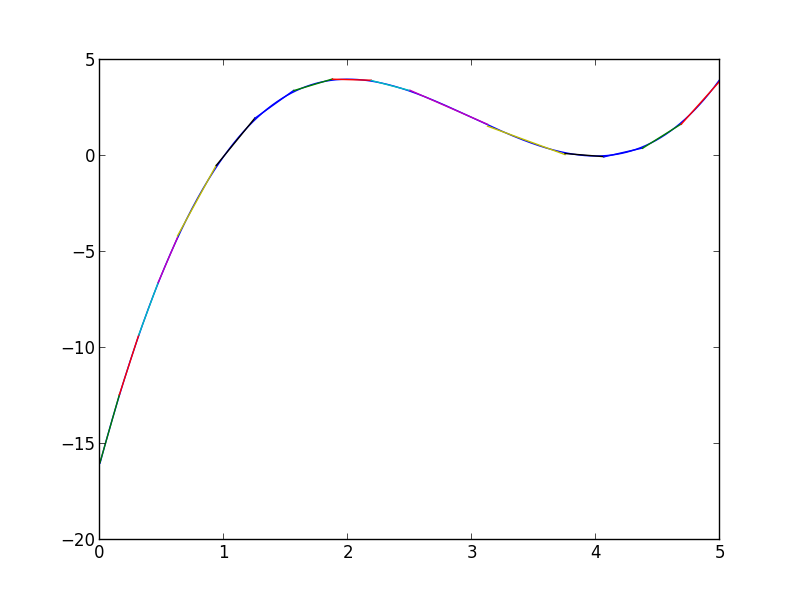
\includegraphics[width=0.5\linewidth]{18.png}
  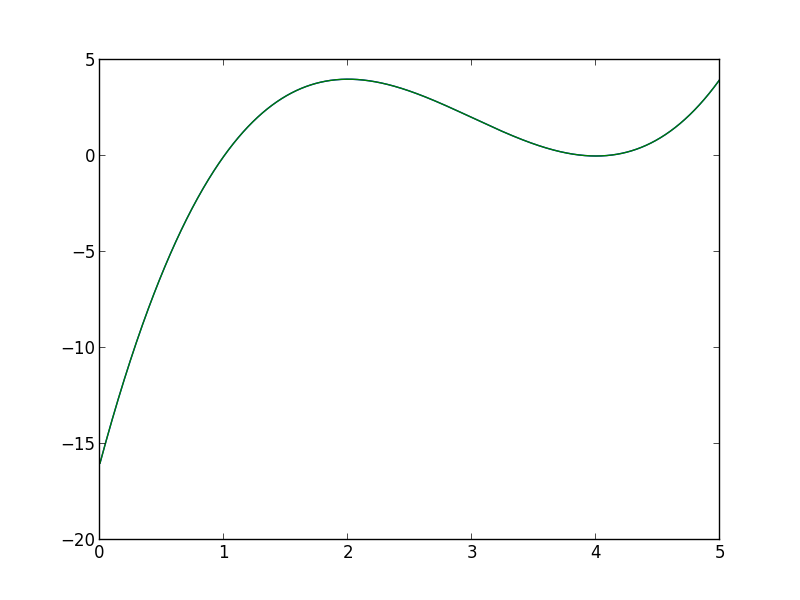
\includegraphics[width=0.5\linewidth]{28.png}}
\end{frame}

\begin{frame}{Wanneer?}
  \begin{itemize}
    \item[\checkmark] Feb, maart: theorie lezen, $\pm 6$ pagina's tekst, implementatie Python \pause
    \item April, mei: theorie op papier, implementatie in C \pause
    \item Daarna: 2-dimensionaal, parallelliseren, toepassen
  \end{itemize}
\end{frame}

\begin{frame}{Jan Westerdiep -- Adaptieve benaderingsmethodes}
  \centering
  \includegraphics[width=0.4\linewidth]{42.png}
  \includegraphics[width=0.4\linewidth]{48.png}\\
  \includegraphics[width=0.4\linewidth]{32.png}
  \includegraphics[width=0.4\linewidth]{38.png}\\
\end{frame}

\begin{frame}{Schets van inhoudsopgave}
  \begin{enumerate}
    \item 1-dimensionale geval \pause
    \item 2-dimensionale geval \pause
    \item Implementatie in C \pause
    \item Parallelliseren \pause
    \item Implementatie in e.o.a.~parallelle situatie (GPU, supercomputer) \pause
    \item (wellicht) Uitbreiding en toepassing
  \end{enumerate}
\end{frame}

\end{document}
